The following sections are dedicated to the Camera Layer of this project. This layer includes Raspberry Pi 2, database, stepper motor drivers, stepper motor, lens, and camera module subsystems. The Camera Layer manages the actions set fourth by the user in the Web Interface layer.

\subsection{Raspberry Pi Subsystem}

\begin{figure}[h!]
	\centering
 	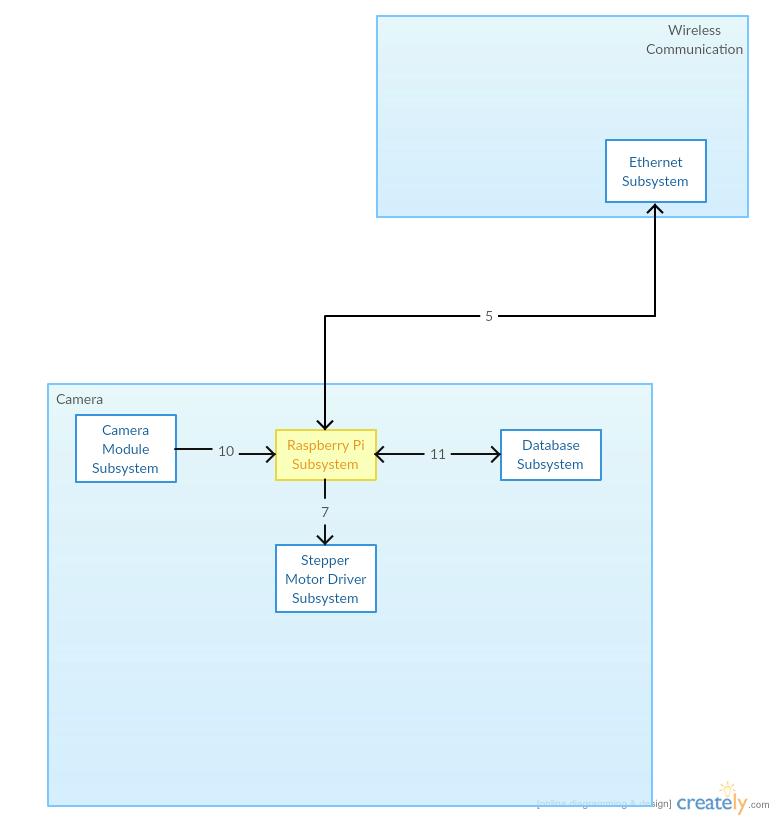
\includegraphics[width=0.60\textwidth]{images/ADS diagrams/raspberrypisubsystem.png}
 \caption{Raspberry Pi Subsystem Description}
\end{figure}

The above diagram illustrates graphically the interaction of the Raspberry Pi Subsystem with other Subsystems from the Camera Layer.

\subsubsection{Assumptions}
The camera layer is assumed to have Ethernet connection and web interface prior to controlling the camera and its movements. Stepper motor and camera module are physically hard wired to the Raspberry Pi. 

\subsubsection{Responsibilities}
The Raspberry Pi 2 is controlled by user input in the web interface layer, which is then responsible for controlling all other subsystems in the camera layer.

\subsubsection{Subsystem Interfaces}

\begin {table}[H]
\caption {Subsystem interfaces} 
\begin{center}
    \begin{tabular}{ | p{1cm} | p{6cm} | p{3cm} | p{3cm} |}
    \hline
    ID & Description & Inputs & Outputs \\ \hline
    \#5, 7, 10, 11 & Controls all other subsystems in the camera layer/bus & \pbox{3cm}{Ethernet \\ Module \\ Database } & \pbox{3cm}{Stepper motor drivers \\ Database}  \\ \hline
   
    
    \end{tabular}
\end{center}
\end{table}



\subsection{Database Subsystem}

\begin{figure}[h!]
	\centering
 	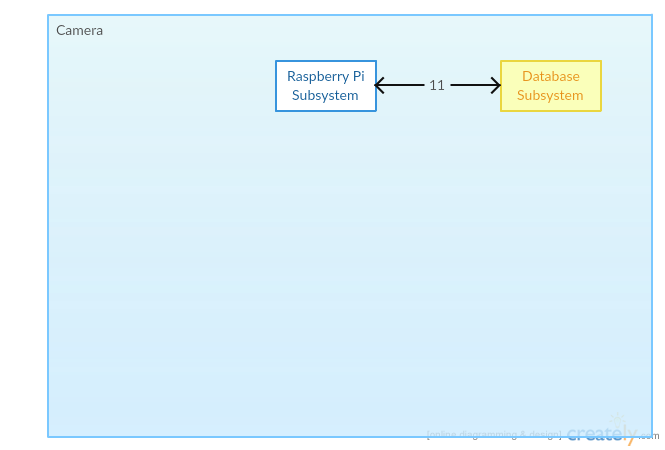
\includegraphics[width=0.60\textwidth]{images/ADS diagrams/databasesubsystem.png}
 \caption{Database Subsystem Description}
\end{figure}

The above diagram illustrates graphically the interaction of the Database Subsystem with the Raspberry Pi Subsystem.

\subsubsection{Assumptions}
The camera layer is assumed to have Ethernet connection and web interface prior to controlling the camera and its movements.  

\subsubsection{Responsibilities}
The Rpi 2 has Ethernet connection, so all the information sent and received by the Raspberry Pi is stored in the database, which is used to store logs of important information.

\subsubsection{Subsystem Interfaces}

\begin {table}[H]
\caption {Subsystem interfaces} 
\begin{center}
    \begin{tabular}{ | p{1cm} | p{6cm} | p{3cm} | p{3cm} |}
    \hline
    ID & Description & Inputs & Outputs \\ \hline
    \#11 & Keep user interaction logs/bus & \pbox{3cm}{Raspberry Pi } & \pbox{3cm}{Raspberry Pi}  \\ \hline
   
    
    \end{tabular}
\end{center}
\end{table}






\subsection{Camera Module Subsystem}
\begin{figure}[h!]
	\centering
 	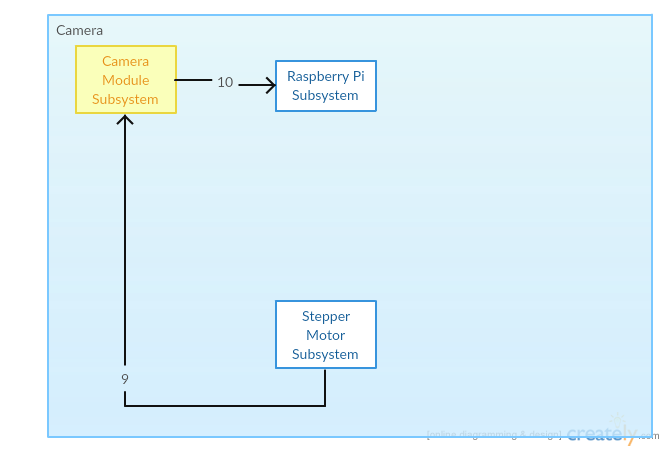
\includegraphics[width=0.60\textwidth]{images/ADS diagrams/cameramodulesubsystem.png}
 \caption{Camera Module Subsystem Description}
\end{figure}

The above diagram illustrates graphically the interaction of the Camera Module Subsystem with the Raspberry Pi and Stepper Motor Subsystems.

\subsubsection{Assumptions}
The camera layer is assumed to have Ethernet connection and web interface prior to controlling the camera and its movements. The camera module is hard wired to the Raspberry Pi.  

\subsubsection{Responsibilities}
The lens is mounted to the camera module. The camera module is then controlled by the stepper motor, which moves the camera (pan and tilt) certain degrees based on user interactions. The camera module is responsible for capturing images of the surrounding landscape.

\subsubsection{Subsystem Interfaces}

\begin {table}[H]
\caption {Subsystem interfaces} 
\begin{center}
    \begin{tabular}{ | p{1cm} | p{6cm} | p{3cm} | p{3cm} |}
    \hline
    ID & Description & Inputs & Outputs \\ \hline
    \#10, 11 & Campture images/bus & \pbox{3cm}{Stepper motor } & \pbox{3cm}{Raspberry Pi}  \\ \hline
    
    
    \end{tabular}
\end{center}
\end{table}





\subsection{Lens Subsystem}
\begin{figure}[h!]
	\centering
 	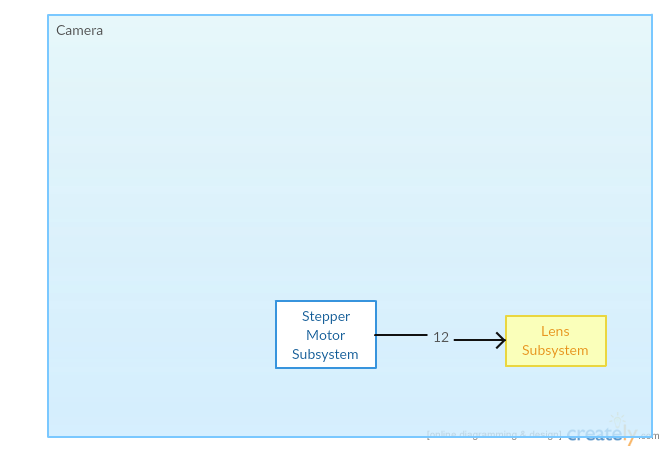
\includegraphics[width=0.60\textwidth]{images/ADS diagrams/lenssubsystem.png}
 \caption{Lens Subsystem Description}
\end{figure}

The above diagram illustrates graphically the interaction of the Lens Subsystem with the Stepper Motor Subsystem.

\subsubsection{Assumptions}
The camera layer is assumed to have Ethernet connection and web interface prior to controlling the camera and its movements. The lens is physically mounted on to the camera module.  

\subsubsection{Responsibilities}
The lens is responsible for providing camera quality images. The lens is mounted to the camera module. The camera module is then controlled by the stepper motor, which moves the camera (pan and tilt) certain degrees based on user interactions.

\subsubsection{Subsystem Interfaces}

\begin {table}[H]
\caption {Subsystem interfaces} 
\begin{center}
    \begin{tabular}{ | p{1cm} | p{6cm} | p{3cm} | p{3cm} |}
    \hline
    ID & Description & Inputs & Outputs \\ \hline
    \#12 & Improve camera quality images/bus & \pbox{3cm}{Stepper motor } & \pbox{3cm}{N/A}  \\ \hline
    
    
    \end{tabular}
\end{center}
\end{table}






\subsection{Stepper Motor Driver Subsystem}
\begin{figure}[h!]
	\centering
 	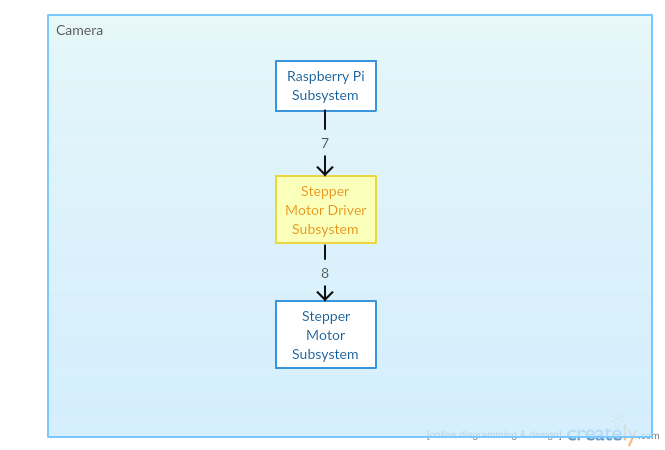
\includegraphics[width=0.60\textwidth]{images/ADS diagrams/steppermotordriversubsystem.png}
 \caption{Stepper Motor Driver Subsystem Description}
\end{figure}

The above diagram illustrates graphically the interaction of the Stepper Motor Driver Subsystem with the Raspberry Pi and Stepper Motor Subsystems.

\subsubsection{Assumptions}
The camera layer is assumed to have Ethernet connection and web interface prior to controlling the camera and its movements.  

\subsubsection{Responsibilities}
The stepper motor driver is essentially software installed on the Raspberry Pi to control the stepper motors and allow the stepper motors to work.

\subsubsection{Subsystem Interfaces}

\begin {table}[H]
\caption {Subsystem interfaces} 
\begin{center}
    \begin{tabular}{ | p{1cm} | p{6cm} | p{3cm} | p{3cm} |}
    \hline
    ID & Description & Inputs & Outputs \\ \hline
    \#7, 8 & Allow stepper motors to work/bus & \pbox{3cm}{Raspberry Pi } & \pbox{3cm}{Stepper Motor}  \\ \hline
   
    
    \end{tabular}
\end{center}
\end{table}






\subsection{Stepper Motor Subsystem}
\begin{figure}[h!]
	\centering
 	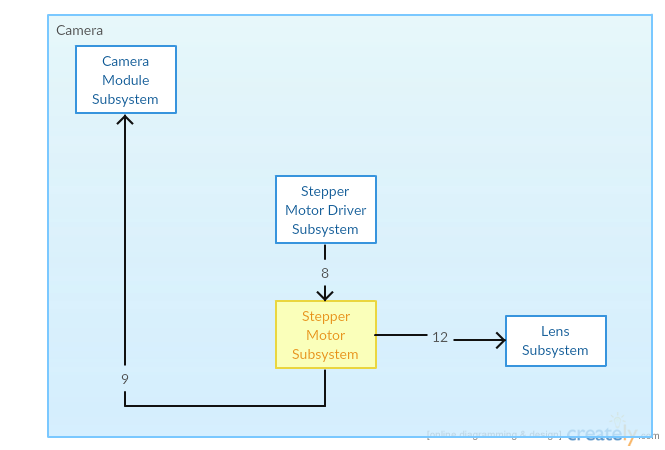
\includegraphics[width=0.60\textwidth]{images/ADS diagrams/steppermotorsubsystem.png}
 \caption{Stepper Motor Subsystem Description}
\end{figure}

The above diagram illustrates graphically the interaction of the Stepper Motor Subsystem with the Stepper Motor Driver, Lens, and Camera Module Subsystems.

\subsubsection{Assumptions}
The camera layer is assumed to have Ethernet connection and web interface prior to controlling the camera and its movements. The Stepper Motor is physically hard wired to the Raspberry Pi. 

\subsubsection{Responsibilities}
The stepper motor driver is essentially software installed on the Rpi2 to control the stepper motors. The stepper motors are connected to the GPIO in the Rpi2 through wires. The lens is responsible for improving camera quality images. The lens is mounted to the stepper motor which moves based on user interaction. The camera module is also controlled by the stepper motor, which moves the camera (pan and tilt) certain degrees based on user interactions.

\subsubsection{Subsystem Interfaces}

\begin {table}[H]
\caption {Subsystem interfaces} 
\begin{center}
    \begin{tabular}{ | p{1cm} | p{6cm} | p{3cm} | p{3cm} |}
    \hline
    ID & Description & Inputs & Outputs \\ \hline
    \#8, 9, 12 & Control lens and camera module/bus & \pbox{3cm}{Stepper motor driver} & \pbox{3cm}{Lens \\ Camera Module}  \\ \hline
   
    \end{tabular}
\end{center}
\end{table}

